\section{Arbeitsaufwand}
\subsubsection{Soll}

\begin{table}[H]
	\centering
    \begin{tabular}{|p{6cm}|p{6cm}|}
    \hline    
    \rowcolor{lightblue}
	Phase & Aufwand \\ \hline   
	Inception & 1 Woche \\ \hline
	Elaboration & 2 Wochen \\ \hline
	Construction1 & 3 Wochen \\ \hline
	Construction2 & 3 Wochen \\ \hline
	Construction3 & 3 Wochen \\ \hline
	Construction4 & 3 Wochen \\ \hline
	Transition & 1 Woche \\ \hline
	\rowcolor{lightblue}
	Total & 14 Wochen \\ \hline
    \end{tabular}
    \caption[Zeitplanung]{Zeitplanung}
\end{table}
\medskip
Um den Aufwand über die ganze Projektdauer ausgeglichen zu verteilen rechneten wir mit:
\begin{itemize}
    \item Aufwand pro Woche: 52 Stunden
    \item Aufwand geplant Total: 52 Stunden * 14 Wochen = \textbf{728 Stunden}
    \item Aufwand pro Student: 728 Stunden / 2 = \textbf{364 Stunden}
\end{itemize}

Das Frühlingssemester 2016 an der HSR hat offiziell 15 Wochen  (inklusive Ostern, Auffahrt und Pfingsten). Bis zur Abgabe der Bachelorarbeit, dem 18.06.2016, sind zusätzlich zwei weitere Wochen gegeben. Damit am Ende es Projektes der Aufwand nicht exponentiell steigt, planten wir unsere Stunden über das offizielle Frühlingssemester und hielten uns die restliche Zeit als Reserve frei.
\subsubsection{Ist}
Während des ganzen Projektes haben wir in Jira Phasen geplant, dazu Tasks erstellt und entsprechen Zeit verbucht.

\begin{figure}[H]
	\centering
	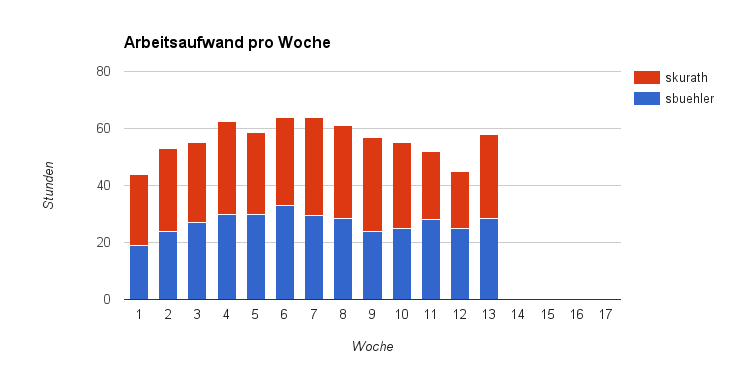
\includegraphics[width=480pt]{images/arbeits_aufwand_pro_woch.png}
	\caption{Arbeitsaufwand pro Woche}
\end{figure}

\begin{table}[H]
	\centering
    \begin{tabular}{|p{6cm}|p{6cm}|}
    \hline    
    \rowcolor{lightblue}
	Student & Aufwand \\ \hline   
	Severin Bühler & 400 Stunden \\ \hline
	Samuel Kurath & 400 Stunden \\ \hline
	\rowcolor{lightblue}
	Total & 800 Stunden \\ \hline
    \end{tabular}
    \caption[Arbeitsaufwand]{Arbeitsaufwand}
\end{table}

\newpage